\documentclass[conference]{IEEEtran}

  \usepackage{booktabs}
  \usepackage{listing}
  \usepackage{amsmath}
  \usepackage{algorithm}
  \usepackage{array}
  \usepackage{url}
  \usepackage{cite}
  \usepackage{complexity}
  \usepackage{algpseudocode}
   \usepackage{graphicx}
   \usepackage{enumerate}
   \usepackage{subcaption}
   \usepackage[shortlabels]{enumitem}


% \usepackage{algorithm}
  \ifCLASSINFOpdf
  
  \else
  
  \fi
  
  \hyphenation{op-tical net-works semi-conduc-tor}
  
  \begin{document}
  
  \title{Parallel Distributed Multi-objective Fuzzy Genetics-based Machine Learning \\ Midterm Report}
  
  \author{\IEEEauthorblockN{Bowen Zheng, Shijie Chen, Shuxin Wang}
  \IEEEauthorblockA{Department of Computer Science and Engineering\\
  Southern University of Science and Technology\\
  Shenzhen, Guangdong, China\\}
  }
  
  \maketitle
  
  \begin{abstract}
  In the second period of the project, we finished the design of fuzzy classifiers, GBML framework and the asynchronous parallel distributed system. We have implemented each part respectively and are working to integrate them together.
  \end{abstract}
  \IEEEpeerreviewmaketitle
  
  \section{Introduction}
  In this project, we aim to build a parallel distributed implementation of a multi-objective genetics based machine learning(GBML) algorithm. We choose a specific problem of a three-objective fuzzy rule-based classifier and fit it into a hybrid GBML framework. Then we develop a parallel mechanism to accelerate computation.

  Code of the three parts have been completed. We will integrate them together, fix bugs and run some test problems in the next stage.

  \section{Fuzzy Rule-based Classifiers}
  The design and implementation of fuzzy classifier is based on \cite{ishibuchi2007analysis}.
  \subsection{Fuzzy Rules}


  \begin{table}[H]
    
    \centering
      \begin{tabular}{cccc}
      \toprule
      Variable&Name\\
      \midrule
      $n$&dimension of patterns\\
      $M$&number of classes of patterns\\
      $S$&a fuzzy classifier\\
      $I$&number of membership functions\\
      $x_p$&a pattern vector\\
      $x_{pi}$&attribute of $x_p$ value on $i$-th dimension\\
      $A_{qi}$&antecedent fuzzy set\\
      $\mu_{A_{qi}}(x)$&membership function of $A_{qi}$\\
      $\mu_{A_{q}}(x_p)$&compatibility grade of $x_p$ with $A_q$\\
      $A_q$&antecedent part of $q$-th rule\\
      
      $R_q$&$q$-th rule\\
      $C_q$&consequent class for $q$-th rule\\
      $CF_q$&rule weight for $q$-th rule\\
  \bottomrule
  \end{tabular}
  \caption{Notation}
  \label{table:1}
  \end{table}
    We use the following "if-then" rules:
\begin{equation}
Rule\;R_q:\;if\;x_{pi}\;is\;A_{qi},\;then\;Class\;C_q\;with\;CF_q
\end{equation}  
Input vectors are normalized to a hypercube $[0,1]^n$ using the following equation:
\begin{equation}x_{pi}=\frac{x_{pi}-min(x_{i})}{max(x_{i})-min(x_{i})}\end{equation}

  The antecedent fuzzy set contains a membership function of the form:
  \begin{equation}
    \mu_{A_{qi}}(x_{pi}) =max\{1-\frac{|a-x_{pi}|}
  {b},0\}
  \end{equation}
  \begin{equation}
    a=\frac{k-1}{K-1}
  \end{equation}
  \begin{equation}
  b=\frac{1}{K-1}
  \end{equation}
  
  where K is the number of intervals of fuzzy set $A_{qi}$ and k is the order of the interval. As shown in Fig.\ref{u0} and Fig.\ref{u3}. The $don't\;care$ condition is a constant function with value 1. As we will discuss in classification process, feature $x_{pi} $ with $A_{qi}$ being $don't\;care$ is ignored by rule $R_q$. 

  \begin{figure}[H]
 	\centering
 	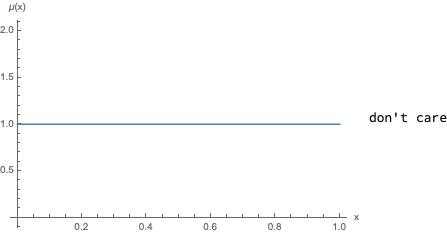
\includegraphics[width=0.4\textwidth]{figures/u1.png}
   \caption{The $don't care$ function}\label{fig:digit}
   \label{u0}
 \end{figure}
 \begin{figure}[H]
 	\centering
 	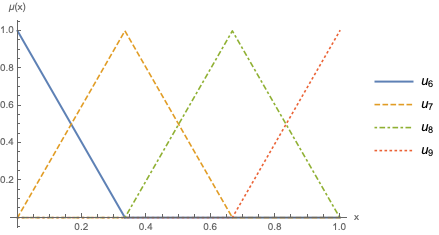
\includegraphics[width=0.4\textwidth]{figures/u4.png}
   \caption{Membership Functions with 4 intervals}\label{fig:digit}
   \label{u3}
 \end{figure}
  The antecedent part of $R_q$ is a set of antecedent fuzzy sets:
\begin{equation}A_q = \{A_{qi}|i = 1,2,...,n\}\end{equation}

  We define the compatibility grade of a pattern $x_p$ with rule $R_q$ as
  \begin{equation}\mu_{A_q}(x_p) = \prod_{i = 1}^{n}\mu_{A_{qi}}(x_{pi})\end{equation}

  The consequent class $C_q$ and rule weight $CF_q$ are decided by the training data used to generate the rule. 
  Assume we have $m$ training patterns $x_{p} \in \{x_{p1},x_{p2},...,x_{pm}\}$ from the $M$ classes. We determine $C_q$ and $CF_q$ as follows:

  First, we compute the confidence of fuzzy rule $R_q$ to each class $c(A_q \Rightarrow Class\;h), h = 1,2,...,M$
\begin{equation}
c(A_q \Rightarrow Class\; h) = \frac{\sum\limits_{x_p \in Class\;h}\mu_{A_q}(x_p)}{\sum\limits_{p=1}^m\mu_{A_q}(x_p)}
\end{equation}

  Then the consequent class $C_q$ as the class with which $R_q$ has the largest confidence.
  \begin{equation}
  \scriptsize c(A_q \Rightarrow Class\;C_q)=max\{c(A_q \Rightarrow Class\;h)|h=1,2,...,M\}
\end{equation}
  
  Rule weight $CF_q$ of $R_q$ is given by the difference between its consequent class and other classes.
  \begin{equation}
  \scriptsize CF_q = c(A_q\Rightarrow Class\;C_q)-\sum\limits_{h=1, h\neq C_q}^{M}c(A_q\Rightarrow Class \; h)
\end{equation}

  Rule weight $CF_q$  shows the quality of a classification result given by a fuzzy rule. Fuzzy rules with negative rule weight are abandoned.
  
  \subsection{Fuzzy Classifier}
  
  A fuzzy classifier $S$ is a set of fuzzy rules. Given an input pattern $x_p$, the classification result $C_w$ is produced by a winning rule $R_w$, chosen as follows:
  \begin{equation}\mu_{A_w}(x_p) \cdot CF_w = max\{\mu_{A_q}(x_p)\cdot CF_q|R_q\in S\}\end{equation}
  \subsection{Generate Fuzzy Rule From Training Patterns}
  At the initiation stage of our GBML algorithm, the population, set of fuzzy classifiers, is created from training data. We can use certain training patterns to create a fuzzy classifier and repeat the process to create a set of classifiers.
  
  Each rule $R_t$ in each classifier is generated from a training pattern $x_t$ as follows:
% \begin{itemize}
    % \item

  We choose an antecedent fuzzy set according to each $x_{ti}$ and form the antecedent part $A_t$ of rule $R_t$ so that $x_{t}$ has the largest compatibility:
  \begin{equation} \A_{ti} = \underset{\mu_j}{\arg\max}\{\mu_{j}(x_{ti})\},j=1,2,...,I\end{equation}
    % \item 
  
  Then, randomly change the antecedent fuzzy set to $dont't\;care$ according to a pre-specified probability $p_{dc}$. This step prevents overfitting and improves generalizing ability of fuzzy rules.
% \end{itemize}
  \section{Hybrid Genetics-based Machine Learning Framework}
  After designing the fuzzy classifier, the next step is to approach our three objectives: maximizing number of correctly classified training patterns, minimizing number of fuzzy rules and minimizing total number of antecedent conditions in the fuzzy classifier S. Our current implementation only consider first two objectives.
	 
	 We use a hybrid GBML algorithm to find the non-dominated rule sets. The genetic algorithm we used is based on \cite{ishibuchi2007analysis}. This hybrid GBML is implemented in the framework of non-dominated sorting genetic algorithm II(NSGA-II) and it's a Pittsburgh-style algorithm. Besides,it use Michigan-style GBML to change a rule as the mutation operation. 
	 
  In our genetic algorithm, the population is a set of fuzzy classifiers, and each individual is a single fuzzy classifier. The basic steps of our algorithm are:
  \begin{enumerate}
  \item Initialize the population with size $N_{pop}$ using training data.
  \item Generate $N_{pop}$ offsprings by crossover operation. Then apply mutation on the offsprings.
  \item Combine the original population and offsprings and keep the best $N_{pop}$ individuals according to Pareto ranking and crowding measure.
  \item Repeat 2) and 3) until the stopping criterion is met.
  \end{enumerate}
  
	 
	 \subsection{NSGA-II}
	 
   NSGA-II, which is a common algorithm for multi-objective optimizing problems, is introduced in detail in \cite{996017}. Compared to ordinary genetic algorithms, it uses elite-preserving, Pareto ranking, and crowding measure to control the population. Elite-preserving is a strategy that we keep the individuals with the best performance in each iteration. Pareto ranking and crowding measure are used for non-dominated sorting in the three-objective situation. Individuals are ranked by Pareto-ranking first. If two individuals have the same Pareto-ranking, on with lower crowding measure is preferred.
   
	 \subsubsection{Elite-preserving}
	 
	 Elite-preserving is a replacing strategy. The idea is that we replace individuals with bad performance in the original population by the outstanding offsprings, and keep preeminent parents to reserve their high performance gene. 
	 
	 \subsubsection{Pareto ranking}
	 
   Pareto-optimal front is the solution set that we want to find in the multi-objective optimizing problem, and its definition can been seen at \cite{ishibuchi2007analysis}. Solutions are divided into  non-dominated solution sets where there is no solution dominated by another solution in the set. Pareto ranking are assigned as the number of non-nominated solution sets that dominates it. In particular, the Pareto-optimal front is not dominated and is seen as the set of best solutions.
	 
	 \subsubsection{Crowding measure}
	 
	 Crowding measure is used to find a more evenly distributed Pareto set and maintain the diversity of the population. This will enhance the algorithm's ability to escape local optimal. An individual's crowding measure is computed as the sum of its distances to its neighboring vectors on both positive and negative directions for each objective. Priority is given to individuals with larger crowding measure.
	 
	 \subsection{Michigan-style GBML}
	 
   Different from the Pittsburgh-style algorithm, Michigan-style GBML sees a single fuzzy rule as the population and sees the membership function as an individual. We use Michigan-style GBML as a mutation operator acting on a single rule to add diversity to the population. 
   
  
   
  \section{Asynchronous Parallel Distributed System Design}
  We propose an asynchronous parallel distributed system to accelerate our GBML algorithm. 


  \begin{figure}[H]
    \centering
    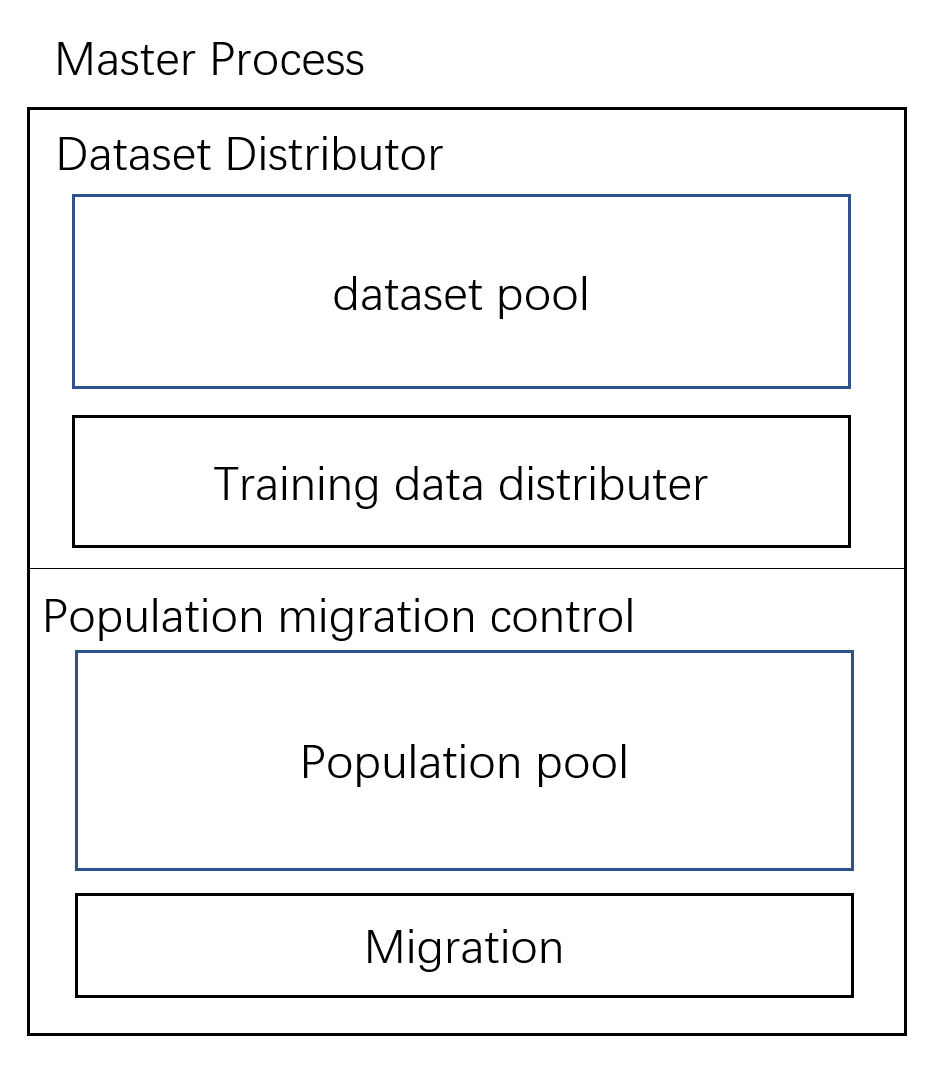
\includegraphics[width = 0.4\textwidth]{figures/master.png}
    \caption{The master process}
    \label{fig:master}
  \end{figure}

  \begin{figure}[H]
    \centering
    \includegraphics[width = 0.4\textwidth]{figures/slave.png}
    \caption{The slave process}
    \label{fig:slave}
  \end{figure}
  
  As shown in Fig.\ref{fig:master} and Fig.\ref{fig:slave}, the model includes 3 parts: dataset distributor, local island worker and population migration control. (For convenience, slave process are referred to as island in this report)
   
  \subsection{Master and Slave process}
  \subsubsection{Master Process}
  
  \begin{enumerate}[leftmargin=4\parindent]
    \item Read dataset and initialize the dataset pool
    \item Distribute $N_{land}$ samples to each island through dataset distributor layer.
    \item Start P slave processes. Each works on a cpu core.
    \item Wait for all islands finish their “init” part and return their population. Use these populations, build an initialized population pool.
    \item Start each islands main part.
    \item Listening each island, exchange(migrate) population on request.
    \item Terminate when receiver a stopping message from all islands.
  \end{enumerate}

  \subsubsection{Slave Processes}\mbox{}
  
  Init:
  \begin{enumerate}[leftmargin =4\parindent]
  \item Receive training dataset from the master process.
  \item Initialize population from the dataset.
  \item Run the GBML for $I_{init}$ iterations.
  \item upload population to the master process.
  \end{enumerate}

  Main:
  \begin{enumerate}[leftmargin=4\parindent]
  \item Run the GBML for $I_{update}$ iterations.
  \item Upload the population to the master process and wait for the new population from migration control layer.
  \item Terminates if stopping criterion is met and sent a stopping message to the master process.
  \end{enumerate}

	\subsection{Dataset Distributor:}
	The dataset distributor is responsible for the dataset distribution process, which delivers a portion of the training dataset to each island as local training data. During this process, the distributor randomly picks $N_{land}$ data from the dataset pool and send it to a slave process. Repeat this procedure for each island.
  \subsection{Population Migration Control:}
  In the initialization stage, the population migration control layer send training data to each island and awaits returned population. When it receives returned population from all islands, it put together these populations and form a large population pool. 
	
	After the initialization, this layer delivers new population to each island on request and activates their “main” part. The new population is generated by randomly selecting $ N_{pop_{i}}$ individuals from the current population pool. Selected data will be deleted from the pool so that the size of the pool remains unchanged.
	
  \subsection{Asynchronous Population Migration}
  After initialization(synchronized), each island will run the GBML algorithm independently for $I_{update}$ iterations and then updates its population through population migration control layer. In this way, population migration of each island is independent and that reduces the barrier time cost. We expect that our model could improve parallel efficiency especially when the update interval of the islands are different. 
  
  
  \section{Computational Experiments}

	 Our current implementation has integrated a two-objective hybrid GBML framework and the fuzzy rule-based classifier. Feasibility test is done on the Iris Flower\cite{Iris} and Gesture Phase dataset\cite{Gphase}. 

   As is shown by Fig.\ref{irisTr} and Fig.\ref{irisT}, the performance on Iris Flowers, which has 4 attributes and 150 instances, is good.
 \begin{figure}[H]
 	\centering
 	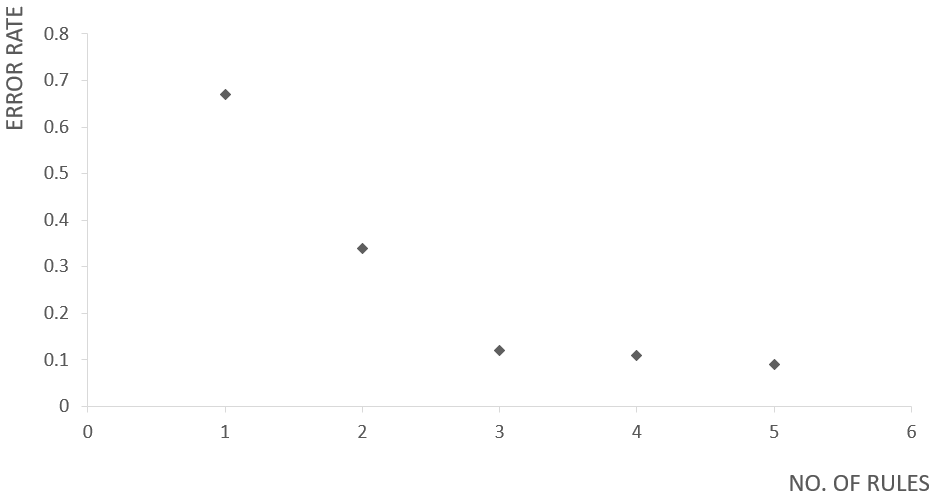
\includegraphics[width=0.4\textwidth]{figures/iris.png}
 	\caption{Performance on training data using Iris Flowers}\label{irisTr}
 \end{figure}
 \begin{figure}[H]
 	\centering
 	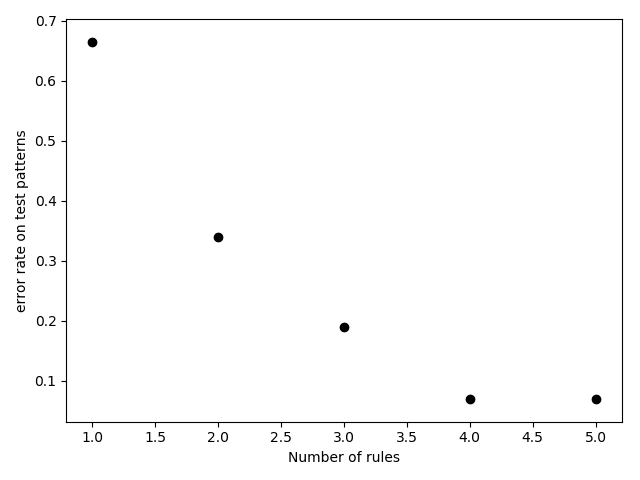
\includegraphics[width=0.4\textwidth]{figures/irisTest.png}
 	\caption{Performance on training data using Iris Flowers}\label{irisT}
 \end{figure}
 
 \begin{figure}[H]
 	\centering
 	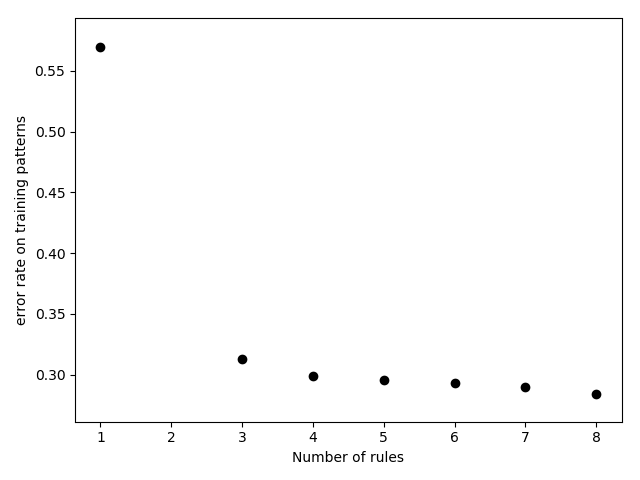
\includegraphics[width=0.4\textwidth]{figures/test.png}
 	\caption{Performance on test data using Gesture Phase}\label{phTr}
 \end{figure}
  \begin{figure}[H]
 	\centering
 	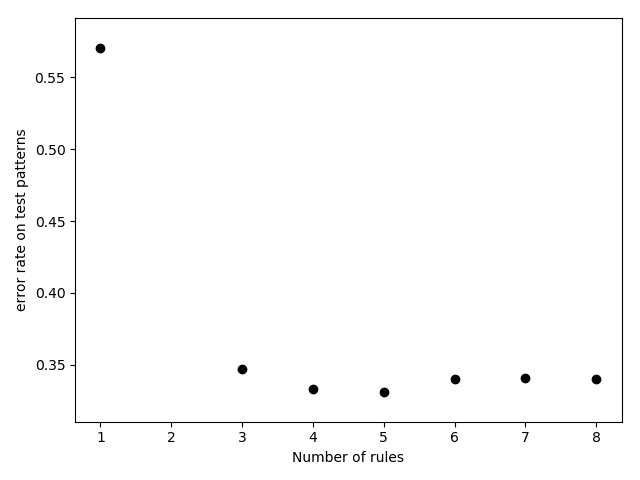
\includegraphics[width=0.4\textwidth]{figures/testData.png}
 	\caption{Performance on test data using Gesture Phase}\label{phT}
 \end{figure}
However, we observe significant performance drop on the Gesture Phase data set as is shown by Fig.\ref{phTr} and Fig.\ref{phT}. The dataset has 32 attributes and 1743 instances.
 \section{Conclusion}
 Currently we have implemented a fuzzy rule-based classifier in a two-objective hybrid GBML framework. We will fix bugs (if any) of the fuzzy GBML algorithm, bring in another objective and integrate the algorithm into our proposed asynchronous parallel system in the final stage of this project. 

  \section{Contribution}
  
    \begin{itemize}
    \item Bowen Zheng - Design \& Implementation of parallel system
    \item Shijie Chen - Design \& Implementation of fuzzy classifier, Design of parallel system
    \item Shuxin Wang - Design \& Implementation of Hybrid GBML framework
    \end{itemize}

\bibliographystyle{ieeetr}
\bibliography{ref}
% that's all folks
\end{document}


  